\documentclass[12pt]{article}
\usepackage{amsmath}
\usepackage{epsfig}
\usepackage{subfigure}
\usepackage{rotating}
\usepackage{fancyheadings}
\input epsf
\setlength{\oddsidemargin}{0.0in}

\setlength{\textwidth}{6.5in}

\setlength{\topmargin}{-0.5in}

\setlength{\textheight}{9.0in}
%
\bibliographystyle{unsrt}

\title{MATFEAP user documentation}
\author{David Bindel}

\pagestyle{fancy}

\headrulewidth 1.5pt
\footrulewidth 1.5pt
\chead{MATFEAP}
\cfoot{\thepage}

\begin{document}

\maketitle

\section{Introduction}

MATFEAP is an interface between MATLAB and the finite element analysis
program FEAP.  Using either the Java Virtual Machine installed with MATLAB
or a C MEX file, MATFEAP communicates with a FEAP server via either a socket
or a pipe:
\begin{center}
  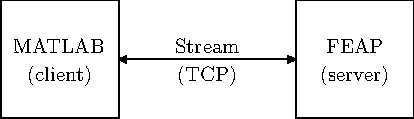
\includegraphics{commfig}
\end{center}

The FEAP server may run on the same machine as the MATLAB client,
or on a different machine altogether.  The server machine does not
need to have MATLAB installed.


\section{Simple example}

To give the flavor for how MATFEAP works in practice, we give a simple
example that uses several of MATFEAP's capabilities.

The {\tt Iblock2} input deck in the example subdirectory describes a
square mesh with {\tt n} elements on a side, where the parameter {\tt n}
is not defined in the input deck.  We start a FEAP simulation with
{\tt n = 10}, get the tangent stiffness and residual into MATLAB,
solve the linear system and write the results back to FEAP, and then
use FEAP's X11 graphics to show the displaced shape.  Once the user
has finished admiring our deformed block, he can press a key (at which
point the FEAP simulation will exit and the graphics will disappear).

\begin{verbatim}
param.n       = 10;  % Parameter to the FEAP input deck
param.verbose = 1;   % See everything that FEAP sends

p  = feapstart('Iblock2', param);  % Start FEAP simulation

K  = feaptang(p);    % Form the tangent matrix
R  = feapresid(p);   % Form the residual force vector
du = K\R;            % Compute a Newton update
feapsetu(p, du);     % Set the displacement vector

% Plot the results
feapcmd(p, 'plot', 'defo', 'mesh', 'boun', 'load', 'end');

% Quit
disp('Press any key to exit');
pause;
feapquit(p);

\end{verbatim}



\section{Building MATFEAP}

To build the FEAP server, edit {\tt makefile.in} in the MATFEAP home
directory and run {\tt make}.  This will build the FEAP pipe server
({\tt srv/feapp}) and the FEAP socket server ({\tt srv/feaps}).

If you wish to use the (non-required) C MEX interface to the network
socket functions, you will also need to type {\tt make cclient}.  You
need not do this if you plan to use the Java interface.  If you wish
to use MATFEAP with Octave -- which does not have a JVM attached --
you can do so with the C MEX interface


\section{Running MATFEAP}

There are three modes for running MATFEAP: pipe, TCP, or UNIX.
The default Java client can communicate with FEAP using a pipe or
a TCP socket; the C MEX client can communicate with FEAP using a
TCP socket or a UNIX-domain socket.  For single-system use, TCP
sockets are relatively slow, so the default behavior is to use
the pipe interface (when running with Java) or the UNIX-domain
socket interface (when running with C).  Of these mechanisms,
the UNIX-domain sockets are fastest on the limited number of systems
where I have done timings.

Before running any simulations, you will need to run the {\tt
  matfeap\_init} script to set the system paths and select the default
communication mode.  This initialization routine should work fine with
MATLAB versions 7+, including the student edition.  In MATLAB 6.5, the
class path used by MATLAB's JVM cannot be dynamically modified, so one
has to set that variable in another way -- see the Mathworks site for
details.


\subsection{Running in pipe mode}

If you wish to use pipe mode (the default mode for the Java client),
you don't need to do anything special.  Just run the desired script:
\begin{verbatim}
  >> matfeap_init
  Using Java socket bindings
  Using FEAP in pipe mode: /home/dbindel/work/feap/matfeap/srv/feapp
  >> cd example
  >> blocktest1
  norm(K*u+R) = 2.01376e-15
  >>
\end{verbatim}


\subsection{Running with UNIX-domain sockets}

If you wish to use UNIX sockets (the default mode for the C client),
you will first need to start the FEAP server.  From the shell prompt,
run {\tt srv/feapu}.  Then open a MATLAB session, and you should be
able to run the desired script.
\begin{verbatim}
  >> matfeap_init
  Using C socket bindings
  Using FEAP on UNIX socket: /tmp/feaps-dbindel
  >> cd example
  >> blocktest1
  norm(K*u+R) = 2.01376e-15
  >> 
\end{verbatim}

If you are testing new elements, you may want to use the {\tt feapu-vg}
script, which runs the FEAP socket server (for a UNIX domain socket) in
{\tt valgrind}.


\subsection{Running with TCP sockets}

If you wish to use TCP sockets, you will first need to start the FEAP
server.  From the shell prompt on the machine where you wish to run
FEAP, run {\tt srv/feaps}.  Then open a MATLAB session, and after running
{\tt matfeap\_init}, use the {\tt feaps\_tcp} command to specify that you
are using a TCP socket server.
\begin{verbatim}
  >> matfeap_init
  Using C socket bindings
  Using FEAP on UNIX socket: /tmp/feaps-dbindel
  >> feaps_tcp
  Using FEAP in TCP mode: 127.0.0.1:3490
  >> cd example
  >> blocktest1
  norm(K*u+R) = 2.01376e-15
  >>
\end{verbatim}

If you are running the client and the server on different machines, you
will need to specify the server hostname as an argument to {\tt feaps\_tcp}.
\begin{verbatim}
  >> matfeap_init
  Using C socket bindings
  Using FEAP on UNIX socket: /tmp/feaps-dbindel
  >> feaps_tcp('box173.cims.nyu.edu')
  Using FEAP in TCP mode: box173.cims.nyu.edu:3490
  >> cd example
  >> blocktest1
  norm(K*u+R) = 2.01376e-15
  >>
\end{verbatim}



\end{document}
